\documentclass[../main.tex]{subfiles}
\graphicspath{{\subfix{../images/}}}
\graphicspath{{\subfix{../equations/rov-model/}}}
\graphicspath{{\subfix{../equations/thruster-model/}}}

% Adicionando comandos matemáticos necessários
\usepackage{amsfonts}
\usepackage{amssymb}

\begin{document}

A fundamentação teórica fundamental para modelagem de ROV é descrita em Fossen (Fossen, 2021), onde é demonstrado o modelo matemático para uma embarcação marítima com 6 DOFs. As equações de movimento adotadas do modelo dinâmico de Fossen contam com a equação de cinemática, equação~\ref{eq1}, e a equação de cinética, equação~\ref{eq2}.
\begin{equation}
    \dot{\eta} = J(\eta)v\label{eq1}
\end{equation}

\begin{equation}
    M\dot{v}+C(v)v+D(v)v+g(\eta)=\tau\label{eq2}
\end{equation}
Onde:
\begin{itemize}
    \item $J(\eta)$ -- É a matriz de transformação entre Body e NED;
    \item $M$ -- É a matriz de massa total;
    \item $C$ -- É a matriz de Coriolis;
    \item $D$ -- É a matriz de amortecimento hidrostático;
    \item $g$ -- É o vetor geral de restauração de força;
\end{itemize}


A equação~\ref{eq1} representa a cinemática do sistema, descrevendo assim os aspectos geométricos da movimentação do ROV em relação a diferentes coordenadas, enquanto a equação~\ref{eq2} representa a cinética do modelo, que consiste na análise de forças e momentos incluídas no ROV durante o movimento.

Baseando-se nas equações de cinemática e cinética para 6 DOFs é possível modelar o sistema do BlueROV light, que só é capaz de se movimentar em 4 DOFs. Dessa forma, os graus de liberdade que não são acessados pelo robô são zerados nas matrizes.

\subsection{Modelo e Alocação de Thruster}
O modelo de ROV utilizado (BlueRov2 light) conta com 6 thrusters, como é possível visualizar na figura~\ref{force_diagram}, sendo esses 4 horizontais e 2 verticais, tendo sua configuração ilustrada também na figura~\ref{force_diagram}. Dessa forma, os thrusters dianteiros (1 e 2) giram no sentido anti-horário e os traseiros (3 e 4) giram no sentido horário.

\begin{figure}[!htb]
  \centering
  \caption{Diagrama de thruster e forças.}
  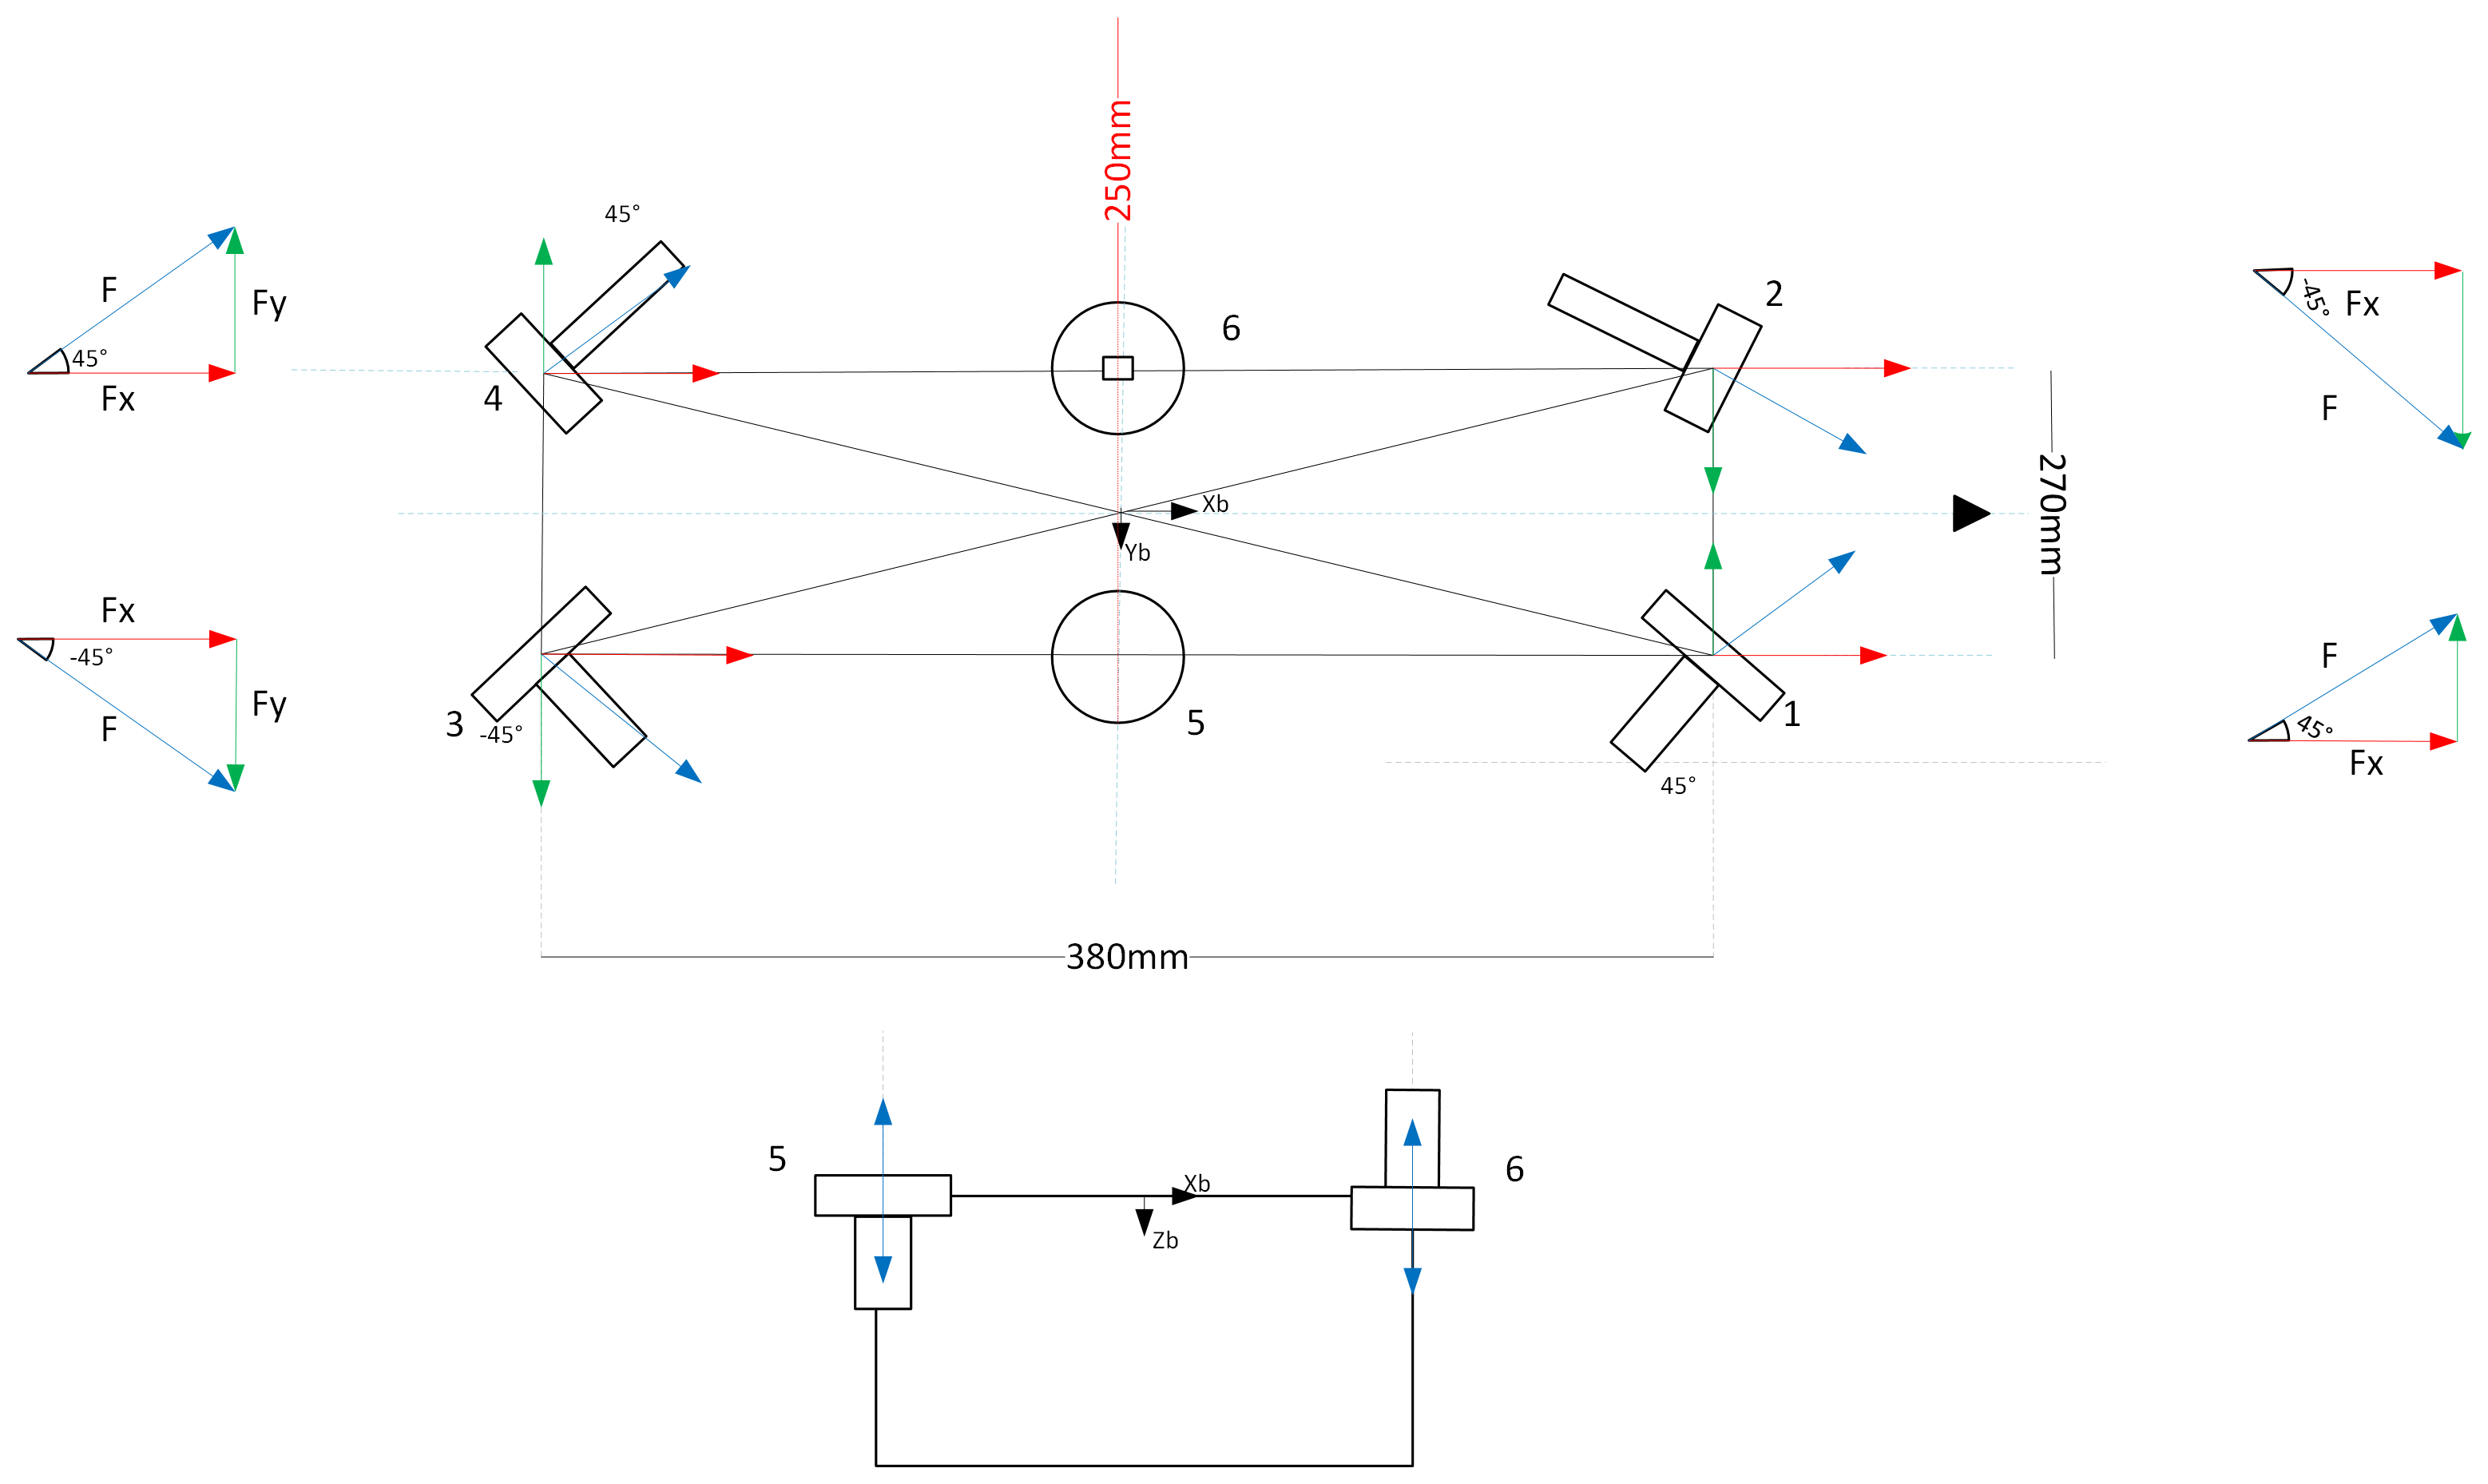
\includegraphics[width=0.45\textwidth]{images/Alocaçao-thrusters-vetor-força-blureov2-light.png}
  \vfill
  Fonte: Autores.
  % \vspace{-\baselineskip}
  \label{force_diagram}
\end{figure}

Apesar da configuração física atípica dos thrusters, posicionados em direções opostas, a alocação de forças foi corretamente realizada graças à rotação em sentidos contrários. Caso todos os thrusters rotacionassem no mesmo sentido, essa disposição geraria forças opostas, comprometendo o controle do sistema. No entanto, como evidenciado na Figura~\ref{force_diagram}, a rotação alternada dos thrusters soluciona esse problema, permitindo a geração das forças desejadas.

Conforme apresentado por \cite{wu20186}, o modelo de um thruster pode ser apresentado de forma linear pela equação~\ref{eq1}. Onde a força do thruster é representada pelo vetor~\ref{force-vector}, os inputs de controle são representados por~\ref{control-input}, e os coeficientes de thruster são representados pela matriz diagonal~\ref{diagonal-K}.

% modelA
\newcommand{\modelA}{%
\begin{equation}
    F = Ku
    \label{one_thruster_force}
\end{equation}
}

% modelB
\newcommand{\modelB}{%
\begin{equation}
    \tau =
    \begin{bmatrix}
    f \\
    r \times f
    \end{bmatrix}
    =
    \begin{bmatrix}
    F_{x} \\
    F_{y} \\
    F_{z} \\
    F_{z}l_{y} - F_{y}l_{z} \\
    F_{x}l_{z} - F_{z}l_{x} \\
    F_{y}l_{x} - F_{x}l_{y}
    \end{bmatrix}
    \label{force-moments-6dof}
\end{equation}
}

\newcommand{\modelfourdofs}{%
\begin{equation}
    \tau =
    \begin{bmatrix}
    f \\
    r \times f
    \end{bmatrix}
    =
    \begin{bmatrix}
    F_{x} \\
    F_{y} \\
    F_{z} \\
    F_{y}l_{x} - F_{x}l_{y}
    \end{bmatrix}
    \label{force-moments-4dof}
\end{equation}
}

% vetorF
\newcommand{\vetorF}{%
\begin{equation}
    F =
    \begin{bmatrix}
    F_{1} & F_{2} & ... & F_{n}
    \end{bmatrix}^{T}
    \label{force-vector}
\end{equation}
}

% vetorU
\newcommand{\vetorU}{%
\begin{equation}
    u =
    \begin{bmatrix}
    u_{1} & u_{2} & ... & u_{n}
    \end{bmatrix}^{T}
    \label{control-input}
\end{equation}
}

% vetorK
\newcommand{\vetorK}{%
\begin{equation}
    K =
    \begin{bmatrix}
    K_{1} & K_{2} & ... & K_{n}
    \end{bmatrix}
    \label{diagonal-K}
\end{equation}
}

% vetorFmin
\newcommand{\vetorFmin}{%
\begin{equation}
    f =
    \begin{bmatrix}
    f_{x} & f_{y} & f_{z}
    \end{bmatrix}^{T}
    \label{given-force-vector}
\end{equation}
}

% vetorR
\newcommand{\vetorR}{%
\begin{equation}
    r =
    \begin{bmatrix}
    l_{x} & l_{y} & l_{z}
    \end{bmatrix}^{T}
    \label{moment-arms}
\end{equation}
}

\newcommand{\vetorRfour}{%
\begin{equation}
    r =
    \begin{bmatrix}
    0 & 0 & l_{z}
    \end{bmatrix}^{T}
    \label{moment-arms-4d}
\end{equation}
}

% generalisedTau
\newcommand{\generalisedTau}{%
\begin{equation}
    \tau = T(\alpha)F = T(\alpha)Ku
    \label{generalised-tau}
\end{equation}
}

% vetorT
\newcommand{\vetorT}{%
\begin{equation}
    T =
    \begin{bmatrix}
    t_{1} & t_{2} & t_{3} & t_{4} & t_{5} & t_{6} & t_{7} & t_{8}
    \end{bmatrix}
    \label{thrusters-config}
\end{equation}
}

% t1Allocation
\newcommand{\tOneAllocation}{%
\begin{equation}
    \tau_{1} =
    \begin{bmatrix}
    F_{1} \cos(\pi/4) \\
    -F_{1} \sin(\pi/4) \\
    0 \\
    F_{1} \sin(\pi/4) \times 0.085 \\
    F_{1} \cos(\pi/4) \times 0.085 \\
    -F_{1} \sin(\pi/4) \times 0.156 - F_{1} \cos(\pi/4) \times 0.111
    \end{bmatrix}
    \label{tau1-allocation}
\end{equation}
}

\newcommand{\tOneAllocationResult}{%
\begin{equation}
    \tau_{1} =
    \begin{bmatrix}
    0.707 \\
    -0.707 \\
    0 \\
    0.06 \\
    0.06 \\
    -0.1888
    \end{bmatrix}
    \label{tau1-allocation-result}
\end{equation}
}

\newcommand{\TpertenceR}{%
\begin{equation}
    T \in \mathbb{R}^{4 \times 6}
    \label{TpertenceR}
\end{equation}
}

\newcommand{\controlinput}{%
\begin{equation}
    u = K^{-1}T^{-1}\tau
    \label{controlinput}
\end{equation}
}

\newcommand{\pseudoinverse}{%
\begin{equation}
    T^{+}=T^{T}(TT^{T})^{-1}
    \label{pseudoinverse}
\end{equation}
}

\newcommand{\controlinputF}{%
\begin{equation}
    u=K^{-1}T^{+}\tau
    \label{controlinputF}
\end{equation}
}

\newcommand{\problemotimization}{%
\begin{equation}
    min_{u,s,\tilde{u}}(s^{T}Qs+u^{T}Wu+\beta\tilde{u})
    \label{problemotimization}
\end{equation}
}

\newcommand{\equesujeita}{%
\begin{equation}
    Tu=\tau+s
    \label{equesujeita}
\end{equation}
}

\newcommand{\uminemax}{%
\begin{equation}
    u_{min}\le u\le u_{max}
    \label{uminemax}
\end{equation}
}

\newcommand{\util}{%
\begin{equation}
    -\tilde{u}\le u_{1}, u_{2}, ..., u_{N}\le \tilde{u}
    \label{util}
\end{equation}
}
\modelA
\vetorF
\vetorU
\vetorK

Considerando o vetor de força $f$ em~\ref{given-force-vector} e o vetor de momentos $r$ em~\ref{moment-arms}, podemos calcular as forças e momentos em 6 DOFs pela seguinte fórmula:
\vetorFmin
\vetorR
\modelB

Considerando a limitação do BlueROV para somente 4 DOFs, é possível ajustar as equações~\ref{moment-arms} e~\ref{force-moments-6dof} para obter as forças em 4 DOFs como desejado. Sendo necessário zerar os momentos que não serão aplicados ao ROV, tendo como resultado então:
\vetorRfour
\modelfourdofs

A alocação de controle é então modelada por:
\generalisedTau
Onde $T$ é a matriz de alocação, onde $T \in \mathbb{R}^{4 \times 6}$ e $\alpha$ é o vetor de ângulos de rotação dos thrusters, onde $\alpha \in \mathbb{R}^{6}$. Como consequência, a matriz de configuração de thruster $T$ pode ser calculada usando a equação~\ref{force-moments-4dof}. Uma vez determinadas as forças e momentos dos thrusters, é possível formalizar o problema da alocação, cujo objetivo é distribuir corretamente os esforços para os propulsores, para realizar a ação de controle desejada.

\subsection{Alocação de controle}

\cite{wu20186} define a alocação de controle como o processo que computa o sinal de entrada do controle $u$ e o aplica nos thrusters, de forma que o controle geral de forças $\tau$ possa ser gerado. Partindo da equação~\ref{force-moments-4dof}, é possível calcular o vetor de entradas de controle através da seguinte equação:
\controlinput

Contudo, levando em conta que a matriz $T$ é uma matriz não quadrática, é aplicada a Moore-Penrose pseudo-inversa $T^{+}$, dada por:
\pseudoinverse

Assim, podemos obter o vetor de entradas do controle por:
\controlinputF

\subsection{Formulação da Otimização}

Em \cite{johansen2005efficient} é sugerida uma formulação de otimização para o problema de alocação de controle. É considerado então o seguinte problema de otimização: 
\problemotimization

A equação~\ref{problemotimization} está sujeita ao seguinte:
\equesujeita
\uminemax
\util

A variável $s$ é o termo que garante a constrição proposta em~\ref{uminemax}, que faz com que o resultado da força generalizada $Bu$ desvie das especificações de $\tau$ caso seja necessário. O segundo termo do critério corresponde ao critério de mínimos quadrados, enquanto o terceiro termo minimiza a maior força entre os atuadores, devido a~\ref{util}. O parâmetro $\beta\ge0$ controla a ponderação relativa desses dois critérios, permitindo que sejam tratados os compromissos entre o uso médio e o pior caso do controle.

\end{document}
